\lfoot{Autor: Raphael Simsek}
\subsection{Analyse und Verbesserung des Fahrstils}

Aus persönlicher Erfahrung geht hervor, dass es bei der Ausbildung zum Fahrer eines Kraftfahrzeugs einigen Verbesserungsbedarf gibt. Häufig kann nicht immer der Fahrlehrer einem Fahrschüler einen nachhaltigen oder wünschenswerten Fahrstil näher bringen. Dies ist nämlich oft ein zeitintensiver Prozess ist. Aus diesem Grund wurden sich Gedanken dazu gemacht, wie man diese Situation verbessern kann.

\subsubsection{Sharing}
Am Beginn des Projektes wurde nach bereits bekannten Systemen gesucht, um seinen Fahrstil nachhaltig zu verbessern. Bei dieser Suche stach die Verbreitung von Apps mit \textit{Sharing}-Funktion heraus. Es gibt nämlich bereits in vielen anderen Bereichen Apps, die sich das \textit{Sharing}-Prinzip zu Nutze machen und damit äußerst erfolgreich Ihre Kunden zu einer Veränderung Ihrer Gewohnheiten bringen \cite{SIMR.CH1-fahrstil-analyse.GewohnheitenLoslassen}. Eines der bekanntesten österreichischen Beispiele ist das App-System von Runtastic \cite{SIMR.CH1-Fahrstil-Analyse.BusinessplanRuntastic}.
Nur im Bezug auf das Autofahren konnte kein derartiges System  gefunden werden.

Zu Beginn des Diplomprojektes gab es folglich keine Möglichkeiten für verbesserungswillige Autofahrer ihren Fahrstil zu verbessern und dies dann sogar zu teilen. 
\newpage
\paragraph{Peer-Pressure} 
\begin{wrapfigure}{r}{0.6\textwidth}\centering
    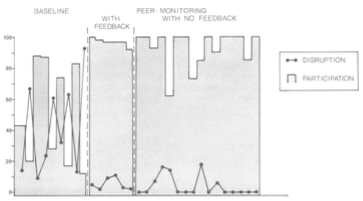
\includegraphics[width=0.6\textwidth]{images/peerPressure}
    \caption{Verhaltensanalyse von Kindern bei gegenseitigem Monitoring \cite{SIMR.CH1-fahrstil-analyse.PeerPressure}} \label{Fig:imgPeerPressure}
\end{wrapfigure}
Das Teilen der Fahrstilanalyse trägt durch \textit{Peer-Pressure}  dazu bei, dass die Nutzer andere Nutzer überbieten möchten und so ihren eigenen Fahrstil verbessern. Diese Theorie bestätigt eine Studie, bei der sich Schüler gegenseitig beobachten. Die Studie zeigt, dass von gleichgesinnten umgebene und überwachte Schüler (hier Social Network) sich selbst angepasster verhalten und sich auf Ihre Vernunft besinnen \cite{SIMR.CH1-fahrstil-analyse.PeerPressure}. Es würden sich Fahrer folglich genauso vernünftiger fahren, wie sich die Schüler in dieser Studie verhalten haben.

Bei der Evaluierung des Project Scope fiel uns besonders auf, dass eine Analyse-Funktion für die nachhaltige Verbesserung des Fahrstils behilflich sein könnte. Es wurde für diese Analyse evaluiert, welche Funktionalitäten am Wichtigsten sind, wobei diese auch innerhalb der Diplomarbeit realisierbar sein sollten.

\subsubsection{Fahrkomfortanalyse}
Eine Analyse der Beschleunigungskräfte, ist üblicherweise nur bei Sportwagen verbaut. Bei derartigen Fahrzeugen wird die Funktionalität nicht für das frühzeitige Verbessern des Fahrstils eines Fahrers verwendet wird, sondern für die Optimierung von Rundenzeiten auf einer Rennstrecke oder schier für das Ausreizen des Möglichen.

\begin{figure}[!htb]\centering
	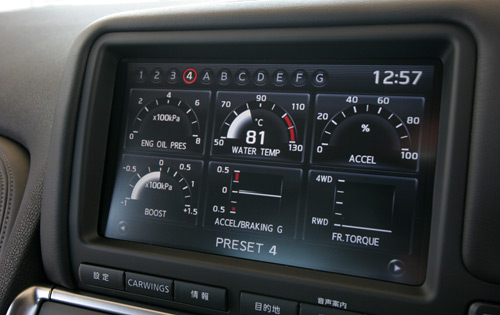
\includegraphics[width=0.6\textwidth]{images/gtrMultifunc}
	\caption{Analyse Möglichkeiten bei einem Nissan GT-R (R35) \cite{SIMR.CH1-Fahrstil-Analyse.GTRMultifunc}}\label{Fig:imgGTR}
\end{figure}

Im Kontrast zu bisher etablierten Möglichkeiten ist die Anzeige der Fahrgastbequemlichkeit anhand fundamental anderen Parametern aufgebaut. Sie soll dem Fahrer aufzeigen welche Kurven dieser zu schnell durchfahren hat. Als Maß für die Bequemlichkeit wird dabei die Beschleunigungskraft in g [Kraft/Masse] herangezogen. Genauere Ausführungen zu diesem Thema, können unter Kapitel 3.5 - Fahrkomfortanalyse gefunden werden.

\subsubsection{Schaltvorschlag}
Der bisherige Schaltvorschlag in einem kostengünstigen, gebrauchten Auto ist oft äußerst simpel gehalten. Es wird hierbei ab einer gewissen Drehzahl der darauffolgende Gang vorgeschlagen oder nur auf den Normzyklus optimiert \cite{SIMR.CH1-Fahrstil-Analyse.Schaltempfehlung}.
\paragraph{Normzyklus}
Der Normzyklus ist insbesondere aufgrund des VW-Skandals bekannt geworden. Es erkennt die Motorsteuerung nämlich, wenn ein Abgastest gefahren wird. Dieser wird in der Fachsprache als Normzyklus bezeichnet wird \cite{SIMR.CH1-fahrstil-analyse.Normzyklus}. Der \textit{modifizierte neue europäische Fahrzyklus (MNEFZ)} ist der Normzyklus, der innerhalb der EU verwendet wird um den Normverbrauch eines Fahrzeuges zu errechnen. Dieser umfasst insgesamt 1180 Sekunden, wovon 780 Sekunden unter Stadtbedingungen und 400 Sekunden über Land gefahren werden. Der MNEFZ wird häufig wegen spritsparender Maßnahmen, vor dem Test, kritisiert. Diese Tricks dürfen von den Autoherstellern eingesetzt werden und umfassen die Erhöhung des Reifendrucks oder das Abklemmen der Lichtmaschine. Ferner wird der Test ohne eingeschalteter Klimaanlage oder anderer \textit{Creature-Comforts} gefahren. Herstellerangaben werden in Europa nämlich selten hinterfragt \cite{SIMR.CH1-fahrstil-analyse.MNEFZ}. In den USA mussten, im Gegensatz dazu, Automobilhersteller bereits in vielen Fällen hohe Entschädigungen zahlen für falsche Verbrauchsangaben bezahlen \cite{SIMR.CH1-fahrstil-analyse.falscherVerbrauchUS}.
\paragraph{Carnot-Prozess}
\todo{sanfter Einführen, wofür brauchen wir den Carnot Prozess}
In diesem musste in Erfahrung gebracht werden, wie ein Motor funktioniert und welche Faktoren diesen beeinflussen. Vor allem ist dabei der Motorwirkungsgrad herausgestochen, welcher mit dem Carnot Prozess definiert ist. Dieser bestimmt wie viel Energie der Motor pro eingespritztem Kraftstoff definiert und ist damit bestimmt damit die Leistung die ein Motor emitiert. Ursprünglich war der Carnot Prozess definiert um einen Kreisprozess zu erläutern und wurde konnte folglich auch auf Motoren angewandt werden.
Der Motorwirkungsgrad nach dem Carnot-Prozess, wird für bekannte Schaltvorschläge in Serienfahrzeugen meist noch nicht verwendet. Der Carnot-Prozess beschreibt die Errechnung des \textit{theoretisch möglichen} Motorwirkungsgrad, ohne dem Hinzuziehen von natürlichen Einflussgrößen. Diese können u.a. Reibung, Temperatur und Dichte sein \cite{SIMR.CH1-Fahrstil-Analyse.CarnotWirkungsgrad}. Genauere Ausführungen zu diesem Thema können im Kaptiel 2.1.2 - Thermodynamik gefunden werden. 

\subsubsection{Schadstoffausstoß}
Eine Live-Messung von \ce{CO2} Werten während der Fahrt ist zumeist eine Schätzung, welche durch den Bordcomputer durchgeführt wird und noch bei wenigen Modellen Einsatz findet. Grenzwerte oder gar eine Analysefunktionalität gibt es in dieser Hinsicht aber nicht. Die \ce{CO2} Werte werden in Zukunft allerdings noch weitaus relevanter. Denn, wie im folgenden Kapitel (1.2 - Umweltbelastung durch \ce{CO2} Ausstoß) ausführlich beschrieben, wird bis 2020 versucht wird einen Durschnittsaustoß von 95 g/km zu erzielen. \cite{SIMR.CH1-Fahrstil_Analyse.EUVerordCO2} Deshalb wurde die Zukunftssicherheit momentaner Bordcomputer in dieser Hinsicht bemängelt.

\subsubsection{Analysefunktion}
Besonders für Fahranfänger kann solch eine Funktionalität von großer Hilfe als lernunterstützendes Medium sein, da momentan ein Fahrschüler nach seiner Fahrstunde nur ein subjektives Feedback seines Fahrlehrers bekommt. Wie ließe sich eine solche Lernunterstützung also umsetzen?
Man könnte dem Fahrschüler am Ende der Fahrstunde eine faktenbasierte Übersicht über seine Leistung während der Fahrstunde geben, welche er dann auch mitnehmen kann und wodurch dieser weiß worauf er bei seiner nächsten Übungsmöglichkeit achten sollte. Die Übersicht soll ausgedruckt oder mittels unserer Webapplikation einsehbar sein (siehe Abb. \autoref{Fig:imgWebapp}). Ausführliche Informationen zur Umsetzung der Webapplikation sind unter Kapitel 3.7 - Webapplikation abrufbar.

\todo{Remove Placeholder image of web application}
\begin{figure}[!htb]\centering
	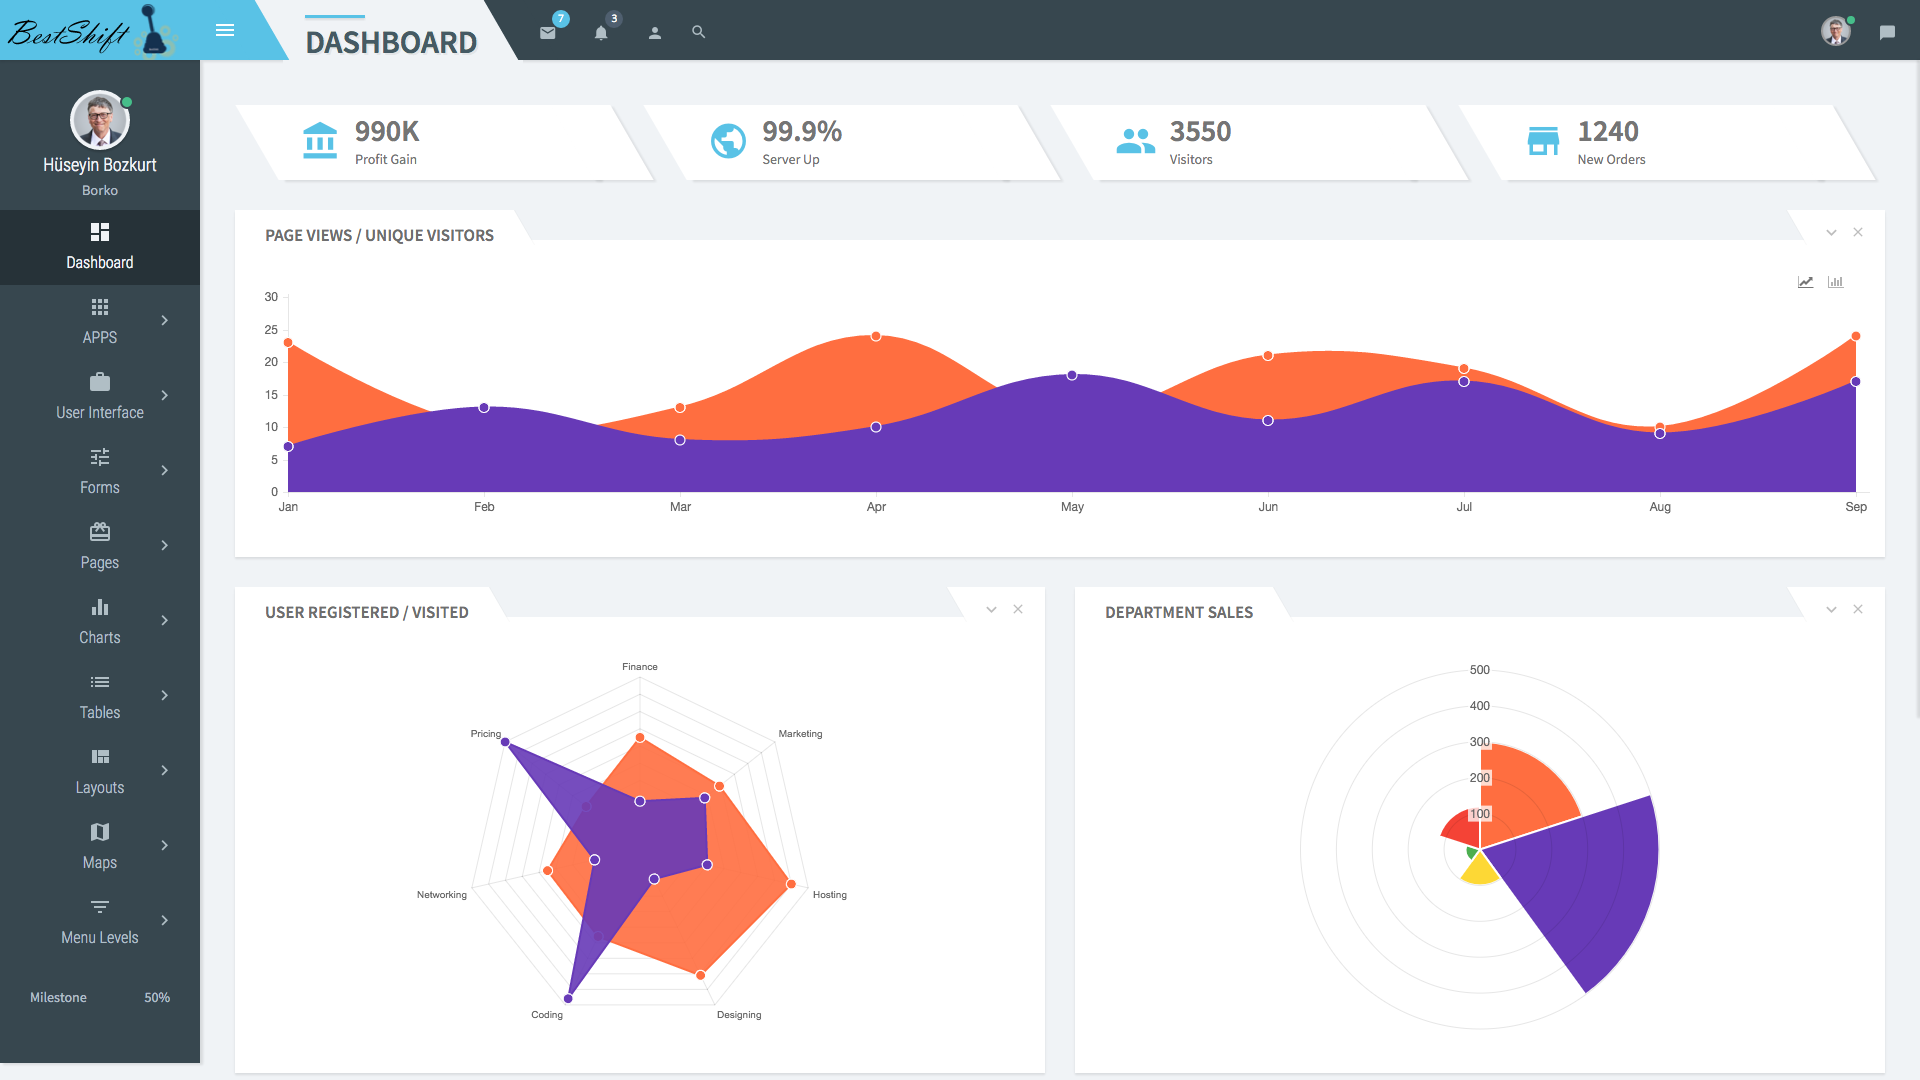
\includegraphics[width=0.6\textwidth]{images/placeholderWebApp}
	\caption{Beispiel Analyse mittels unserer Webapplikation}\label{Fig:imgWebapp}
\end{figure}

Besonders Fahranfänger und Fahrer mit Umweltinteresse könnten die entwickelte Analysefunktionalität gerne nutzen wollen. Die Analysefunktionalität soll besonders für die Zielgruppe eines Fahranfängers aufzeigen, wo der Verbrauch, die Kurvenbeschleunigung (G-Kraft) und die Drehzahl besonders hoch war. Durch diese Daten soll sich der Fahranfänger oder der interessierte Kunde zukünftig verbessern können. Da uns noch kein derartiges System bekannt war, wurde ebenfalls evaluiert ob die Möglichkeiten einer retrospektiven Fahranalyse durch Anbauteile oder Zubehör bereits realisierbar sind.

\paragraph{Car - PC}
Bei der Evaluierung konnte ein Projekt gefunden werden, welches die gelieferten Daten nur in Echtzeit per Computer auslesbar macht. Die Daten werden aber sofort verworfen, weshalb keine retrospektive Analyse mehr möglich wäre. Überdies ist die Programmierung in einer anderen Programmiersprache umgesetzt, weshalb man dieses Projekt keinesfalls auf Android portieren könnte. Das Projekt ist außerdem weitaus teurer (geschätzt €300,-) als von uns gewünscht, denn es wurde überlegt bis zu welchem Preis man sich ein solches Zubehör, auch als normaler Anwender leisten würde, wobei für uns €100,- als Abgrenzung feststand. Daher wurden Überlegungen angestellt, wie man die Idee eines solchen Projektes massentauglicher machen kann und dabei bei geringen Kosten dem Nutzer ein wünschenswertes Erlebnis bieten kann. \cite{SIMR.CH1-Fahrstil-Analyse.LowBudgetCarPC} Dieses Projekt hat uns also geholfen in der Defintionsphase des Projektes Anpassungen vorzunehmen, da es bereits einen Maßstab gab, was im Bereich des Möglichen liegt. Weitere Ausführungen zu dieser Thematik sind unter Kapitel 2.2 - Hardware und Sensorik auffindbar.

Es gibt bisher bei konkurrierenden Echtzeit-Anzeigen (wie. z.B. Torque Pro \cite{SIMR.CH1-Fahrstil-Analyse.TorquePro}) noch keine, wie beschriebene, Analysefunktionalität. Deshalb würde die Analysefunktionalität für einen Autofahrer ein noch nicht etabliertes Produkt darstellen.

\begin{figure}[!htb]\centering
	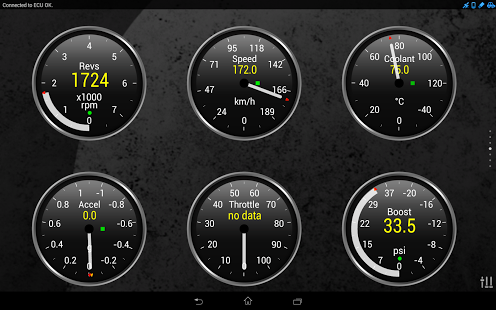
\includegraphics[width=0.6\textwidth]{images/torquePro}
	\caption{Möglichkeiten mit der kostenpflichtigen Torque App  und der OBD Schnittstelle \cite{SIMR.CH1-Fahrstil-Analyse.TorquePro}}\label{Fig:imgGTR}
\end{figure}

Gerade diese Funktionalität würde aber von Fahranfängern benötigt werden um frühzeitig und selbstständig Fehler ihres Fahrstils zu erkennen und auszubessern zu können. Insbesondere konnten wir, unter anderem anhand unserer Erfahrungen, feststellen, dass das Schalten und das gleichmäßige und verbrauchsarme Fahren für viele Fahranfänger eine Herausforderung darstellt. Durch eine Analysefunktion könnten motivierte Fahranfänger mögliche häufige Fehler schneller stoppen und die schlechten Angewohnheiten würden sich nicht im  Gedächtnis eines Fahranfängers verankern. Stattdessen es würden sich, unter regelmäßiger Verwendung der Applikation, bei motivierten Fahrern nur positive Charakteristika gemerkt werden, wie wir bei regelmäßigem Fahren mit einer erfahrenen Person selbst merken konnten. Ferner belegt das Beispiel der gegenseitigen Überwachung durch Schüler \cite{SIMR.CH1-fahrstil-analyse.PeerPressure}, dass Fahrschüler sich gegenseitig motivieren und trainieren könnten.

Eine Analysefunktion in Form einer Webapplikation ist also insbesondere für die Lernkurve bei einem noch ungeübten Kraftfahrzeug-Lenker von großem Vorteil, da diese oft noch nach dem Erhalt des Führerscheins unsicher bezüglich ihres Fahrstils sind und ihnen des Öfteren wiederholt die selben Fehler unterlaufen. Eine genauere Beschreibung der Umsetzung der Web Applikation ist unter Kapitel 3.7 - Web App auffindbar.

\clearpage % DO NOT REMOVE
